\documentclass[11pt]{article}
\usepackage[top=0.70in, bottom=.70in, left=1in, right=1in]{geometry}
\renewcommand{\baselinestretch}{1.1}
\usepackage{graphicx}
\usepackage{natbib}
\usepackage{amsmath}
\usepackage{multicol}
\usepackage{tcolorbox}
\usepackage{caption}
\usepackage{todonotes}
\usepackage[font={sf,footnotesize}]{caption}
\usepackage{hyperref}
\newcommand{\llabel}[1]{\hypertarget{lintarget:#1}{}\linelabel{lin:#1}}

\usepackage{lineno}
\renewcommand\linenumberfont{\normalfont\tiny\color{gray}}


\bibliographystyle{besjournals}

\begin{document}

\title{Closing the gap between statistical and scientific workflows for improved forecasts in ecology}
\date{\today}
\author{Victor Van der Meersch$^{1*}$, James Regetz$^{2}$, T. Jonathan Davies$^{1,3}$ \& EM Wolkovich$^{1}$}
\maketitle
\noindent $^{1}$ Forest and Conservation Sciences, University of British Columbia, Vancouver, BC V6T 1Z4, Canada\\
$^{2}$ National Center for Ecological Analysis and Synthesis, 1021 Anacapa St, Santa Barbara, CA 93101, United States\\
$^{3}$ Botany, University of British Columbia, Vancouver, BC V6T 1Z4, Canada \\
$^{*}$ \url{mailto:victor.vandermeersch@ubc.ca}\\

\noindent \emph{For:} Workflow for Applied Data Analysis theme issue for \emph{Phil Trans A} as an \emph{Opinion}

\begin{abstract}
% Concerns about increasing biodiversity loss and climate change have led to greater demands for useful ecological models and forecasts. Datasets relevant for developing these models and forecasts have also increased in size and complexity, including in their geographical, temporal and phylogenetic dimensions. New research often suggests that models accounting for these complexities can yield more accurate trends and predictions. We argue, however, that the usual workflows for model fitting in ecology make it difficult to evaluate and compare most current models for several reasons. First, the research community is split between two disconnected paradigms: either using data to fit simple, trend-like models with one or few parameters, or developing forecasting models that include complex, mechanistic, and/or black box submodels only indirectly informed by data. Second, in both cases, models tend to be developed not only in isolation of one another, but also without a coherent framework for linking scientific questions and understanding to statistical and modeling decisions, throughout the entire modeling process. We propose a unified, principled workflow for end-to-end empirical model development that bridges the gap between process-based and statistical approaches, integrates sound statistical and scientific practices, and especially relies on data simulation to inform decisions at multiple steps in the process. We argue that this approach, coupled with a shift toward universal training, more open model sharing, and alignment on common datasets, could transform for ecological modeling.
Concerns about biodiversity loss and climate change have led to greater demands for ecological models. Datasets for developing these models have increased in size and complexity, including in their geographical, temporal and phylogenetic dimensions. New research often suggests that models accounting for these complexities can yield more accurate trends and predictions. 
We argue, however, that the usual workflows for model fitting in ecology make it difficult to evaluate and compare current models. First, the research community is split between two spheres that prevent uniting a connection between trend estimation and forecasting. One research sphere focuses on using data to fit simple, trend-like models with few parameters, which is separated from research developing forecasting models, often including complex, mechanistic sub-models indirectly informed by data. Second, in both cases, models tend to be developed without a coherent framework for linking scientific questions and understanding to statistical and modeling decisions. To address these challenges we propose a workflow that integrates statistical and scientific practices through clear steps, many of which rely on data simulation to inform decisions in the process, and where forecasting a natural output. We show how this approach, coupled with a shift toward universal training, more open model sharing, and alignment on common datasets, could harmonize currently divided efforts at trend estimation and forecasting to better inform sustainable policies.

%emw24Jul: I pulled out a few of the best sentences that may help the abstract: I worked some in, see what you think. 
% Implementing sustainable policies to mitigate these impacts is thus a global priority, but designing the best policies requires estimating and understanding biodiversity and ecosystem trends to date, alongside the skill to forecast future dynamics. 
% Towards this aim, we outline the steps of a universal workflow that could harmonize both trend estimation and forecasting.
% Within this workflow, forecasting is a natural output of the process and not a separate process or one available for only certain modeling approaches.
\end{abstract}

% {\noindent \bf Goal:} Increase awareness of how we can merge statistical and scientific workflows in ecology (especially forecasting) and what we would get out of it.
\linenumbers

\section{Introduction}

Anthropogenic drivers are reshaping natural systems \citep{Diaz2019}. Impacts are projected to increase in coming decades, as climate change accelerates biodiversity loss, altering ecosystem services and human well-being \citep{IPBES2019}.
Implementing sustainable policies to mitigate these impacts is thus a global priority, but designing the best policies requires estimating and understanding biodiversity and ecosystem trends to date, alongside the skill to forecast future dynamics. % These requirements in turn have created a growing need for more global ecological data, and the types of models that can robustly handle such data. 

Meeting these \llabel{global}global policy needs has led often to two separate paths: one focused on estimating trends from new global datasets, and another focused on forecasting from generally distinct datasets or mechanistic models based on fewer data. 
Newly available large-scale, long-term datasets have provided our first `global' estimates of biodiversity trends \citep[e.g.][]{loh2005living,Dornelas2018}, but these data---gathered opportunistically from multiple sources---are unbalanced and suffer from large geographic, temporal and taxonomic biases. Models to date have failed to fully address these challenges and, perhaps because of these limitations, are rarely if ever used for forecasting.
Instead, forecasting---under different plausible scenarios---has generally relied on entirely different datasets combined with either correlative or process-based models \citep{IPBES2019}, with process-based models often promoted as the most realistic approach \citep{Urban2016, Pilowsky2022} because they focus on mechanistic representations of ecosystem functioning. These approaches have failed to yield agreement on current species trends, leading to ongoing debates about the magnitude and even direction \citep{Dornelas2014, Leung2020, Buschke2021, Johnson2024}, and producing forecasts that diverge due to high model uncertainty at the ecological level \citep{Cheaib2012, Thuiller2019}.
 
\llabel{inferentialgoal}These two modeling approaches may appear to pursue independent inferential goals---explanation vs.\ prediction---but in reality this distinction is blurred. Trend estimation may be nominally focused on explanatory outcomes, yet it rarely links clearly to theories that could provide causal inference, usually because it tends to be carried out using simpler models. Moreover,  estimated trends are frequently treated---implicitly and explicitly---as quantities that project forward into the future, taking on a forecasting role. 
In contrast, approaches using complex forecasting models are certainly built for predictive purposes, yet these also have an additional agenda. Developing and using mechanistic, process-based models is often justified by the assumption that ``we must understand to predict", and such models are often judged by how faithfully they mimic the real-world processes they represent, which conflates explanation with prediction \citep{Shmueli2010}.

We argue that many current debates and diverging forecasts are driven by the incoherent and disconnected workflows used today in ecology \citep{Loreau2022, Talis2023, Johnson2024}. Research estimating biodiversity trends has become focused on methodological aspects because the current workflow fails to examine the gap between ideal and available data, and rarely tests for predictive accuracy that could scale up to allow forecasting. At the same time, process-based models developed for forecasting often evolve through the addition of new separate layers or components because the current workflow rarely examines the model as a functioning whole and thus ignores major problems (e.g. non-identifiability, discussed below). Thus, it encourages new parts that are often disconnected from the original research aim, its data stream, and the previous scientific insights. 

Workflows that fully integrate all the steps required to build a model from an ecological question, with evaluation of limitations and potential problems before estimating its parameters and making projections, could reduce many of these problems. In particular, we argue that workflows that incorporate data simulation at multiple steps can quickly identify flaws in model structure and constraints in data, and allow us to understand when, where, and why different models diverge \citep{McElreath2018, betanworkflow,Gelman2020,Schad2020,grinsztajn2021,vandeschoot2021,Wolkovich2024}. Towards this aim, we outline the steps of a universal workflow that could harmonize both trend estimation and forecasting.

\begin{figure}
	\centering
	\includegraphics{../../figures/figure_modeldataspaces_revised2}
	\caption{Different trajectories of current (b-c) and proposed (d) workflows through model-data space during model development, from pre-model/pre-data to post-model/post-data quadrants.
	Panel A serves as a legend, showing where model development should begin (carefully thinking about the hypotheses to test) and when inference should be made, for either explanatory purpose (estimation) or forecasting (prediction).
	Panel B illustrates that, in current trend estimation approaches, most time is spent in the post-model/post-data quadrant, where models are directly fitted to empirical data---often with no prior evaluation of the model.
	Panel C illustrates the typical process-based model development where a lot of time is spent building and calibrating (fitting) separate submodels (represented by the separated ovals) without clear distinction between model building and model calibration and without evaluating the full model structure a priori. Additionally, the specific hypotheses the model is designed to test are rarely clearly stated.
	Panel D illustrates the workflow highlighted in this paper (see main text and Figure 2 for details). Ideally, it begins in the pre-model/pre-data quadrant, where the research question is defined. The next step moves to the post-model/pre-data quadrant, where a model is built---independently of the data. This is where we should spend a good deal of time evaluating model behavior using simulated data. Once we are satisfied with our model, we can move to the post-model/post-data quadrant, where the model is fitted to real data. Then, we perform retrodictive checks to compare model predictions to observations, which likely give us some feedback to refine our model.}
	\label{fig:modeldata}
\end{figure}

\section{Scientific method and workflows}

Quantitative science relies on a model-based framework to confront hypotheses with data \citep{Chamberlin:1965cd}. In an idealized scientific method, we would formulate a research question and hypotheses, design an experiment accordingly, build a model, collect data, and use this data to inform our model and differentiate between hypotheses. This method underlies much of the recent pre-registration movement, where hypotheses and methodology are defined prior to data collection \citep{Nosek2018}.
But this idealized method often does not apply to the reality of ecological research. Many important questions cannot be addressed through controlled experiments and replications. In such cases, we must rely on existing, heterogeneous datasets alongside uncertain and incomplete theory to provide a large-scale and long-term perspective \citep{Hilborn1997}. Indeed, most macroecological insights have emerged from exploring patterns in these datasets (exploratory data analysis).

\llabel{robust} This reality should drive researchers to use more coherent methods that remain robust for the intended inferential goals, even with imperfect data and knowledge gaps. But the current workflows combined with the challenges ecologists are facing---both in terms of data complexity and societal needs---instead may lead to persistent problems.
Trend estimation has focused mostly on fitting a model to empirical data (\llabel{quad1}i.e. post-model/post-data, Figure \ref{fig:modeldata}b)---without the checks (\llabel{quad2}post-model/pre-data) and likely feedbacks that often highlight uncertainty and related limitations in the model and/or data (Figure \ref{fig:modeldata}b). For forecasting, researchers have focused on making predictions with increasingly complex mechanistic models (Figure \ref{fig:modeldata}c), frequently obscuring the steps underlying model building and parameterization (\llabel{quad3}and without a clear distinction between pre- and post-data). Researchers often calibrate the different parts of these models separately, and fix some parameter values based on experiments and expert knowledge, to avoid problems when trying to fit the model as a whole.
Addressing these problems while accounting for the realities of working with ecological data requires a more comprehensive workflow.

We argue a workflow that moves \llabel{quad4}along the data-model space in a coherent sequence of steps (Figure \ref{fig:modeldata}d) could reduce many of these problems and thus improve ecological science.
The first step of this workflow is to define an explicit research question and formulate hypotheses (step 1, Figure \ref{fig:workflow}). This involves making clear assumptions about the most influential drivers, within the specific context of our study. This should guide the construction of a narrative model of how we believe the system works, focusing on the mechanisms that could generate the data we observe, including the observational error (\llabel{quad5}pre-model/pre-data, Figure \ref{fig:modeldata}d).  
\llabel{causalinf} This step of carefully formulating hypotheses has gained increasing attention in the ecological literature \citep{Grace2020}. From this narrative, we can then develop a mathematical model---an ensemble of equations that encapsulates our knowledge and is designed to answer our research question (step 2, Figure \ref{fig:workflow}). Generally, starting with a relatively simple model that we could refine later makes understanding the model and how it interacts with empirical data easier \llabel{exampleworkflow1}(see example workflow we provide as a supplementary file). At this stage, prioritizing biologically meaningful parameters is crucial, as it allows us to have a sense of plausible parameter values. This means choosing a model formulation where each parameter corresponds to an interpretable behavior (which sometimes requires considering alternative parameterization). 

With a model in place, the next step focuses on testing and understanding it via data simulation (step 3, Figure \ref{fig:workflow}). `Fake' or `test' data are generated directly from the model by fixing parameters \llabel{firstsim}to some reasonable values, which is straightforward if the parameters are interpretable, and from `fake' (simulated) predictor data. 
We then fit our model to this simulated dataset and evaluate its ability to recover the prescribed values (\llabel{quad6}post-model/pre-data, Figure \ref{fig:modeldata}d). At this stage, the focus is on understanding the model, so we may need to spend time thinking about whether each parameter is realistic or not. This is also a step for making sure the model is working as expected (see example workflow). \llabel{repeatsim} Ideally, this data simulation step should be repeated several times with different parameter values, sampled within a reasonable range. \llabel{priorPC} In a Bayesian framework, simulated parameters can be sampled from the prior distribution (allowing us to check the implications of our priors \citealp{Gelman2020}, \llabel{SBC}and to validate model inferences using simulation-based calibration \citealp{Talts2018_SBC}). In other frameworks, they can be sampled from a range of biologically reasonable values (which is very similar to the concept of a prior).

\begin{figure}[h]
	\centering
	\vspace*{-0.4cm}
    \hspace*{-1.5cm}
	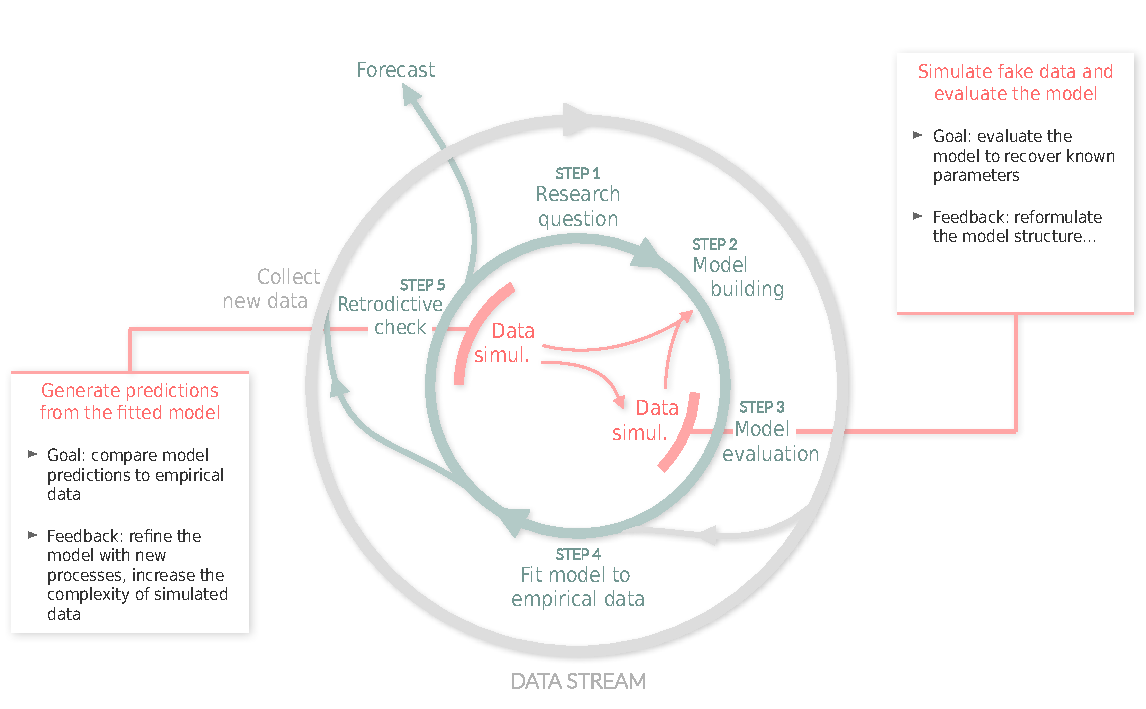
\includegraphics{../../figures/figure_worflow_wsteps}
	\caption{The workflow we propose here, which builds from recent advances in workflows \citep[][]{betanworkflow,Gelman2020,Schad2020,grinsztajn2021,vandeschoot2021,Wolkovich2024}, focuses on iterative feedbacks between the research question, model and data. Most research should start at Step 1, with the research question, followed by extensive model building and evaluation using simulated data (Steps 2 and 3) before proceeding to fitting the model on empirical data and examining it through retrodictive checks (Steps 4 and 5). Within this workflow, forecasting is a natural output of the process and not a separate process or one available for only certain modeling approaches.  The integration of observations (the data stream) occurs at Step 4---only after the model has been thoroughly evaluated---and can also highlight opportunities to collect new data and enrich the data stream. This figure is expanded from Figure \ref{fig:modeldata}d.}
	\vspace*{-0cm}
	\label{fig:workflow}
\end{figure}

Once we are confident about our model structure, we can introduce real data as part of an initial model fitting step (step 4, Figure \ref{fig:workflow}). This way, we obtain parameter estimates constrained by observations (\llabel{quad7}post-model/post-data, Figure \ref{fig:modeldata}d). 
These parameter estimates lead to the second data simulation step, this time using our fitted model parameters to generate predictions (step 5, Figure \ref{fig:workflow}). This---which we call a retrodictive check (\citealp{betanworkflow}, also called a \llabel{PPC}posterior predictive check in a Bayesian workflow,  \citealp{Gelman2020})---allows model output to be compared to observations \llabel{suppfig1}(see Supplementary Figure 1). \llabel{howtoPPC} This is a powerful approach, in part because checks should be tailored to assess key features of the data and model output together in regard to our research question, but this also means there is no standard way to do this \citep{Gelman2020}.
It is only once all steps have been completed that we can interpret parameter values with respect to our research question.
The workflow encourages a focus on the full model, where any parameter (such as a trend estimate) must be carefully interpreted alongside others, as all are fundamental components that shape both inference and forecasting. 

Within such a workflow, forecasting emerges as a natural outcome. Rather than being a final goal, forecasting only involves jointly modeling new circumstances along with the original data. This workflow could also bridge gaps in certain areas between exploratory analyses and developing research questions. For example, in macroecological studies model building is often informed by patterns in the data. The adoption of this workflow would make the exploratory stage more transparent---as an explicit preliminary step for entering the workflow---and would compel researchers to more clearly develop a research question before extensive model fitting (Figure 1). 

A key feature of this workflow is the central role of data simulation, which introduces two feedback loops.
The first feedback arises when we evaluate the model on simulated data.
The failure of the model to recover known parameter values and handle the complexity of the simulated data should prompt reconsidering the model, or even reformulating the research question.
Further, this step might reveal that some parameters are highly non-identifiable (meaning the parameter(s) cannot be uniquely estimated), flagging the need to change the model structure---before incorporating empirical observations. 
The second feedback loop comes from the retrodictive check. 
Discrepancies here may indicate a missing key driver, and suggest the current model is too simplistic. We can refine the model to integrate the missing process(es)---if we can identify them---and return to the start of the workflow. Insights from the retrodictive check can also lead us to introduce additional complexity when simulating fake data, such as phylogenetic structure \llabel{suppfig2}(see Supplementary Figure 1) or observational biases (e.g. unbalanced data). For example, if a researcher realizes their empirical data is geographically biased, this bias should be built into the model and thus into this data simulation step. This iterative evaluation of the model moves beyond a simple reliance on goodness-of-fit metrics. At each iteration, we are able to evaluate the model behavior, both with simulated and real data, taking into account our expert knowledge of the ecological processes. \llabel{broadcontext}These feedback loops are applied currently only in Bayesian frameworks (to our knowledge), but could and should extend across other modeling approaches given their power to improve models and, in turn, scientific understanding.

\section{The workflow in practice}

Across the different fields of ecology---for both parameter estimation and forecasting---a systematic application of a coherent workflow could highlight the best opportunities to accurately \llabel{quant1}understand and manage uncertainties and yield new scientific insights. This will help refocus the debate on designing new hypotheses, formulating new questions---and guiding efforts to collect new data. Here, we illustrate how such a workflow could lead to significant improvements in two related areas: (i) estimating global biodiversity trends and (ii) forecasting species and ecosystem dynamics using process-based models.

\subsection{Trends}

Ecologists today have amassed data on populations and species across the globe; they have also engaged in an increasing number of debates on regional and global trends over time, with arguments over the magnitude and even direction of population and biodiversity metrics \citep{Dornelas2014,Leung2020,terry2022no,muller2024weather}. While shifting estimates are part of the process of science---refining our approaches and thus estimates over time---we believe these debates would be fewer and they would be more rapidly resolved through use of an improved workflow. % Further, an improved workflow could give more rapid and coherent estimates, which could make it easier for  policy-makers to develop and advance initiatives aimed at slowing declines.

We argue that an improved workflow that required data simulation and retrodictive checks would lead to larger model advances and a greater recognition of uncertainty---thus highlighting likely consistency in estimates across models---that could better aid policy.  Using the workflow would make it more obvious that what now appear as major discrepancies are shifts in point estimates that are generally all in the same uncertainty space \citep{Johnson2024}---and it would challenge modelers to show major predictive advances, which is not currently part of the process. Explanatory power in most models of observational data is usually very low \citep{low2014rising,moller2002much} and thus tests of models' predictions rarely expected. But the workflow highlights that predictions from the model---what we call retrodictive checks---are part of the process of science, and critical to testing for what may be missing in a model \llabel{suppfig3}(see Supplementary Figure 1). 

We expect retrodictive checks on most published trend analyses would highlight major missing components in these models, and drive changes both in the models themselves and in the simulated data to check the models. This step builds somewhat on the skills needed for null models \citep{Gotelli:2012oz}, but with a shift in focus towards the specific bespoke model at hand. Ecologists have started to use simulated data more to understand potential limitations of their models and data combined \citep{Hilborn1997}, but this is still extremely rare, and efforts to date often treat simulations as separate from the statistical model \citep{Buschke2021,dove2023quantifying}, short-circuiting their full utility if used in an iterative workflow.

Applying the workflow to current trend estimates could importantly highlight the best way to improve data collection for more reliable estimates. Returning to the example of a global estimate of trends in vertebrate populations of species over time (see Box) and applying our proposed workflow would mean more efforts to define the goal and question---is it a simple global estimate?
Or a need to also find which species are declining most, including those that may have poor or no data? From there a generative model using simulated data for testing could incorporate many aspects of the populations, and data, that are often only included in `null' or `synthetic data generation' currently \citep{Buschke2021,mcrae2025utility}, but could be built into the models fit to the empirical data. Eventually fitting the empirical data and performing retrodictive checks would likely highlight major missing components of the generative model \llabel{suppfig4}(see Supplementary Figure 1) and, ultimately, this would help inform our global estimates of mean trends \llabel{exampleworkflow2}(see example workflow we provide as a supplement file). For example, certain populations are recovering for very specific reasons (e.g. elephants in regions where the ivory trade drove declines in the past) that perhaps should be modeled. From this model, what data are most critically needed to address the updated aims would become clearer and could drive new data collection \citep{toszogyova2024mathematical}. 

\subsection{Forecasting from process-based models}

Ecological forecasting is a broad field with a diverse range of methods. Across these methods, process-based modeling is often considered the gold standard for forecasting in ecology \citep{Urban2016, Pilowsky2022} and beyond because it is based on mechanistic understanding that should drive accurate out-of-sample predictions.  
This focus on a mechanistic basis, however, generally drives newer models to incorporate greater complexity---and an ever-growing number of parameters. This can make it difficult to increase scientific understanding \citep{Franklin2020} and suggest or model potential policies. 
In principle, increasing model complexity can be beneficial by enhancing mechanistic realism, better representing more complex dynamics, and \llabel{quant2}reducing uncertainty by restricting the effective parameter space. In practice, however, this is not always the outcome. In process-based modeling for climate forecasts, the uncertainty range on the effect of increasing CO$_{2}$ concentration on temperature have remained largely unchanged over decades of increasing model complexity \citep{Zelinka2020}. This has driven calls for more rigorous and transparent calibration processes \citep{balaji2022general}. Similar concerns arise in ecology, where strong disagreements persist about the effect of climate change on future species distributions \citep{Cheaib2012} and ecosystem dynamics \citep{Lovenduski2017} after decades of modeling work.
These uncertainties have large implications beyond ecology, as they influence simulations of biosphere-atmosphere interactions and, ultimately, future climate projections \citep{Bonan2018, simpson2025confronting}.
Some researchers now advocate for simplifying models, to avoid over-parametrization when the data provide little information to constrain some parameters \citep{Wang2017, Harrison2021}. These arguments stress that the strength of process-based models is their interpretability, and thus their parameters should represent biological processes, and the values of these parameters are of interest.
If a model becomes too complex, however, it may become a black box, \llabel{blackbox}where many parameters are effectively hidden and can take on unreasonable values. 
Further, with so many parameters, understanding the sources of uncertainty and how they propagate through the model may become nearly impossible (see Box).
Each additional process and parameter can increase overall uncertainty to the point where model projections lose their usefulness for decision makers \citep{Saltelli2020}. 

Process-based models used to project species and ecosystem distributions are some of the most important for informing policy, and they highlight many of these problems. Most of the focus is on the model projections---often represented as values on maps, presented without uncertainties. Model evaluation generally focuses on how well these projections match observed distributions, sometimes under different climatic conditions to challenge the models \citep{VanderMeersch2025a}---most of the time evaluating only one of the many output variables of the model.
The complexity of these models can make it difficult to assess how well the potential parameter space was searched, and whether there was any potential non-identifiability. Studies of such underlying problems are generally separate; thus potential model problems are usually exposed only later \citep{VanderMeersch2025b}, as opposed to being discovered in preliminary steps before generating forecasts. 

Applying the workflow to process-based models would help open the black box and thus could identify and fix model problems before forecasting.
Each successive step of model development in the proposed workflow may highlight problems and a path to solutions. Incorporating data simulation would introduce a crucial step between model building and data fitting (also called calibration), ensuring a clear delineation between the two, and help expose potential parameter identifiability issues earlier in the model design. 
Uncovering identifiability issues would likely force researchers to begin with a simpler version of the model, which they could build on iteratively, testing for support---or lack thereof---when adding model complexity. The workflow may also highlight model problems by requiring more explicit model calibration (i.e. data fitting), which is currently hidden within opaque `model building', making it easy to hide non-identifiability. Once found, non-identifiable parts of models could be addressed by reformulating the mathematical structure of certain processes, or finding ways to apply additional constraints (e.g. narrower ranges for certain parameters or developing new hypotheses that target the appropriate level of complexity). The resulting process-based models would likely be simpler and thus more tractable for quantifying parameter uncertainty and propagating uncertainty through to projections. 

% Box
% \setlength{\columnseprule}{0.1pt}
\begin{tcolorbox}[
sharp corners=all,
colback=white,
colframe=black,
size=tight,
boxrule=0.1mm,
grow to left by=+1cm, grow to right by=+1cm,
enlarge top by=-1.2cm,
left=3mm,right=3mm, top = 2mm, bottom = 2mm,
fontupper=\footnotesize
]
{\begin{multicols}{2}

\centerline{\bf Trend estimation} 
\vspace*{2mm}
\begin{minipage}[t]{\linewidth}
    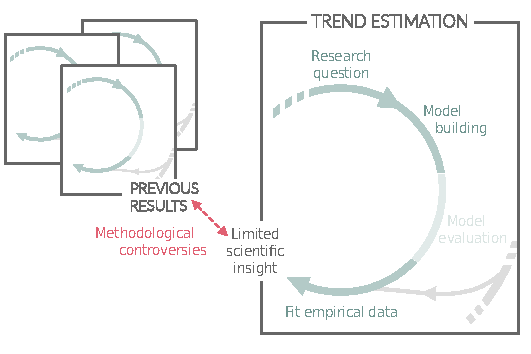
\includegraphics[width=\linewidth]{../../figures/trendestimation_details}

    % \vspace{-0.5cm}\captionsetup{font=footnotesize}\captionof{figure}{Caption}\label{fig:trends}
    \vspace*{1mm}
\end{minipage}

% Trends - outline current problem
% In the current workflow for estimating trends over time, a new model with a new estimate often leads to a paper (see figure A above) because ecologists spend less time interrogating their models with simulated data, or their model performance fit to empirical data.
In the current workflow for estimating trends over time, a model is typically chosen a priori to fit to data, yielding parameter estimates that are treated as true and often translated directly into published findings and conclusions, without interrogating the model using simulated data and carefully evaluating its performance (see example workflow we provide as a supplementary file). Any such analysis must be treated with caution, because different model variants can yield very different estimates (hence different conclusions), and published results may not prove robust when confronted with future reanalysis of the same data (see Figure A above).
The Living Planet Index (LPI, \url{www.livingplanetindex.org}), which aims to include long-term data on vertebrate populations of species across the globe, is emblematic of these conflicting results. % \todo[]{could highlight how influential the LPI has become (recent reports suggest a 73\% ave. pop decline since 1970. This would be massive!}
% With updated data released semi-annually alongside new datasets and new estimates of decline, 
A growing number of high-profile papers have challenged how strong the evidence is for population decline \citep{Dornelas2014,gonzalez2016estimating,wagner2021insect,muller2024weather}, with each paper taking a slightly different analytical approach. For example, using LPI data, \citet{Leung2020} published a mixture model that suggested most populations were not significantly declining, followed by other alternative modeling approaches \citep{Buschke2021,puurtinen2022living} including a recent one suggesting a basic analysis of the dataset should always include three sources of autocorrelation, finding trends that encompassed many previous results \citep{Johnson2024}. 


\vfill

\columnbreak

\centerline{\bf Mechanistic forecasting}
\vspace*{2mm}
\begin{minipage}[t]{\linewidth}
    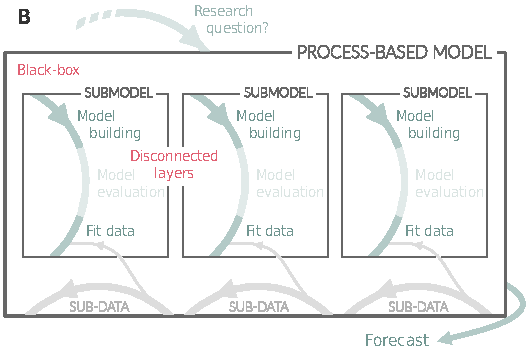
\includegraphics[width=\linewidth]{../../figures/forecasting_details}

    % \vspace{-0.5cm}\captionsetup{font=footnotesize}\captionof{figure}{Caption}\label{fig:trends}
    \vspace*{1mm}
\end{minipage}

\noindent % Process-based models are built on explicit mathematical equations to describe (supposedly causal) relationships between environmental drivers and ecological responses. 
% They also often incorporate empirical relationships, particularly when knowledge is incomplete or when some processes are intentionally omitted. Processes are often represented at different nested spatiotemporal scales, depending on the underlying assumptions. 
Model development is the central step of the process-based workflow, typically requiring several years, yet it often remains opaque for anyone who has not worked the model itself. The step of designing the model---translating knowledge and hypotheses into mathematical equations and parameters---is often blurred with the step of model calibration (or tuning), where parameter values are inferred. Models are often treated as an accumulation of multiple submodels, each governing one or several ecological processes (see Figure B above). Rather than being fitted as a whole, submodels are calibrated separately against specific subsets of data, and some parameters are simply prescribed (i.e., fixed to a value found in the literature) or tuned to reproduce certain observations or theory. The way models are currently calibrated is likely not a coincidence, but rather a workaround to avoid confronting the full complexity of the model. Calibrating submodels separately makes it easier to avoid the likely reality that, if the submodels were fitted together (as a whole), many parameters would compensate for one another---revealing structural degeneracies and making the model far more difficult to use.  %emw24Jul: nice stuff here. 

\vfill

\end{multicols}}

\centerline{\bf A common workflow to bridge trend estimation and forecasting} 
\vspace*{-3mm}
{\begin{multicols}{2}
\begin{minipage}[t]{\linewidth}
	\vfill
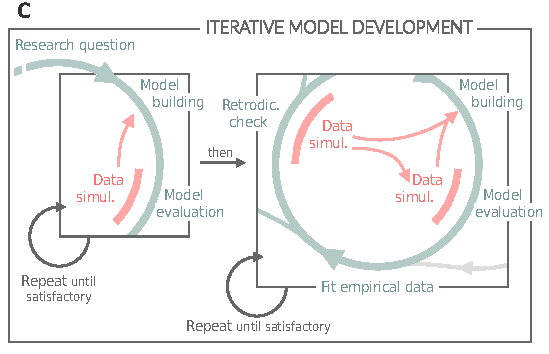
\includegraphics[width=\linewidth]{../../figures/iterativeworkflow_details_revised}
\vfill
% \vspace{-0.5cm}\captionsetup{font=footnotesize}\captionof{figure}{Caption}\label{fig:trends}
\vspace*{3mm}
\end{minipage}

\columnbreak
\vspace*{1mm}
A universal workflow offers an opportunity to bridge statistical and process-based frameworks, integrating mechanistic knowledge and leveraging robust statistical approaches \citep[e.g.][]{rounce2020quantifying}. Process-based models would no longer be perceived as deterministic black boxes by other researchers but rather as robust statistical frameworks encapsulating both data structure and mechanistic knowledge---and where the full model is fitted jointly. It would be an opportunity to incorporate mechanistic assumptions beyond the process-based modeling community, potentially improving trend estimates. For both trend estimation and forecasting, the workflow would refocus attention on the research question, highlighting the ecological hypotheses that justify the use and design of the model.

\end{multicols}}

\end{tcolorbox}

\clearpage
\section{Barriers and opportunities}

We believe our workflow could help advance ecological science and its applications, but widespread use of it requires overcoming major hurdles that pervade science.  
The first is pressure to publish quickly, which can be at odds with the reality that good model fitting is inherently iterative and takes time. The second is reluctance to embrace adoption of open science practices that ensure modeling efforts are fully transparent and reproducible. 
We believe adopting a workflow such as the one we propose may change this reluctance, and aligns with ongoing efforts to place increasing value on research that is carefully developed, openly collaborative (including both data and code), and transparent about areas of uncertainty.

\subsection{Adopting the workflow}

Advancing ecology to where most researchers use models built more flexibly from ecological theory and insights applied to their ecological systems will not happen rapidly without a major shift in training. Much of ecology still divides the world into training for those who gather data and learn a limited set of pre-built models versus those who develop more complex models. In ecological training today, researchers who conduct field and lab studies often learn a limited set of particular statistical tests matched to particular experiment designs and simple information on their variable types (e.g. categorical $x$ and $y$ leads to using a chi-squared test).

When ecologists trained in a limited set of tests require more complex models, they are expected to collaborate with other ecologists \llabel{collab1} trained more in model development (though often for highly specific applications, such as wildlife population estimates, where generative models are often predefined). These two groups further differ from process-based modelers, who often train in physical and ecophysiological processes and how to abstract them into mainly deterministic models.
None of these groups have fully integrated data simulation into their statistical or scientific workflows. Simulation is generally reserved as a form of training needed mainly by those specializing in theoretical ecology, who often solve analytical equations but rarely link to empirical data. While specialization is valuable, we argue the fundamental % training
separation in ecology has overly-siloed these groups and prevented more rapid progress.

% We suggest unified training in our proposed workflow, or a similar one \citep{betanworkflow,Gelman2020, grinsztajn2021,vandeschoot2021}, would focus on learning to generate questions and then models, and then how to simulate data from them. 
We recommend that scientists who regularly engage in model-driven research efforts would benefit from unified training about how to generate well-formed questions and appropriate models, and then how to simulate data from them. Through this and the use retrodictive checks, most ecologists would be better equipped to think through what parameters are most critical to their question and/or aim (e.g. management), and also gain a much stronger connection to the level of uncertainty in many of ecological estimates. Empiricists would be more likely to recognize critical gaps in current models fit by those specializing in ecological modeling and help advance those models. Process-based modelers may start a new generation of simpler models that are more tractable to theoretical ecologists, who may see new bridges from their work to empirical data and forecasting. \llabel{collab}Such progress could be accelerated through collaboration with statisticians who are already using or otherwise well-equipped to adopt our proposed workflow \citep{betanworkflow,Gelman2020, grinsztajn2021,vandeschoot2021}. %emw24Jul: I would say they actually have to be good at doing science to be useful collaborators -- a point Andrew makes often but I think we are tacitly saying that already in second half of this sentence. 

% New paragraph by Jim!
\llabel{studydesignandmore}Beyond routine application of the workflow and universal training to support it, the full transformative potential of the workflow hinges on additional broader systemic changes within the research community. First, fostering more open model sharing through standardized repositories and collaborative platforms would accelerate scientific discovery by allowing researchers to build upon, validate, and refine existing models more efficiently, Second, open sharing of more comprehensive study design and sampling design details associated with datasets would enable more appropriate data integration and model design decisions, and independent validation of these decisions by the community. Third, where feasible, alignment on common datasets would provide a standardized basis for model development and comparison, reducing the fragmentation of efforts and facilitating more direct and meaningful evaluations of different modeling approaches. Coupled with universal training, these shifts in the sharing and standardization of data and models would create a more collaborative, efficient, and rigorous environment for ecological modeling, ultimately leading to more accurate forecasts and better understanding of complex environmental systems.

%emw24Jul: Bold proposed changes below.... see what you think. 
% \subsection{[Need a better title] A tractable alternative to machine learning}
\emph{Conclusions:} 

With rapid advances in machine learning, improving current methods to gain greater scientific insights to drive better forecasting seems increasingly important. \llabel{clearerML} A careful and coherent workflow is essential to preserve the interpretability of non–machine-learning models---their primary advantage. \llabel{MLvsPBM}Machine learning will likely surpass process-based models for forecasting accuracy, especially if the latter lack a robust estimation of their parameters and fall in a complexity trap---a trap with additional costs to interpretability of process-based models. Similarly, estimates of trends from empirical data using models without clear mechanistic drivers may soon offer fewer advantages over machine learning. 

%emw24Jul: I feel like we say most of this before, so suggest we cut it. 
% Beyond improving model building and evaluation, our proposed workflow also has the potential to shift how process-based models are perceived, particularly by those unfamiliar with them.
% Process-based models could once again be a way to answer a research question---whereas today, model simulations have increasingly become a subject of study on their own.
% Ideally, applying the workflow would help to move away from the traditional process-based model paradigm, where parameters are typically assigned fixed values without properly accounting for their uncertainty. Instead, it would guide a step-by-step model fitting, parameter estimation, and uncertainty quantification---preventing modelers from making biased inferences and unfounded assumptions beyond what the data can support. It would thus define a clear and limited context in which the model should apply, and limit discussion of adding increasing complexity. 

Today model development in ecology is rarely transparent, which limits how easily the research community can understand models, and thus identify potential issues. Instead of broad inclusive conversations about how to improve models to advance our ecological understanding, a significant portion of scientific debate has become mired in methodological considerations. However, we believe our workflow provides a tractable step to fixing this. By focusing on model development more tightly tied to ecological expertise, we argue this workflow should broaden the community that contributes to model development. It may also help resolve apparent conflicts by identifying where divergences in model predictions emerge, whether from differences in assumptions, model structures, or other aspects of the modeling process.
As ecologists are increasingly expanding their computational toolkits, many field, and lab, and other forms of `empirical' ecologists have the basic tools to follow this workflow to build models that better represent their ecological domains of interest, and---most importantly---to interrogate those models.

% This shift would present a significant challenge---as it would likely reveal many issues related to non-identifiability in models and data limitations before achieving robust inference. But ultimately, it would prevent modelers from making biased inferences and unfounded assumptions beyond what the data can support.

\clearpage
\bibliography{../../forecastflows.bib}

\end{document}
